\section{Final Specifications and Requirements}
The functional and non-functional requirements the system should meet are given in Table 3.1.All answers should include the following specifications:The whole system must be calibrated to uncertainty, and context labels must be provided and must be attributed to the source.must be easily reproducible on commodity hardware.

\begin{table}[H]
\centering
\caption{Functional (F) and non-functional (N) requirements.}
\label{tab:requirements}
\renewcommand{\arraystretch}{1.2}
\begin{tabular}{|c|c|p{10cm}|}
\hline
\textbf{ID} & \textbf{Type} & \textbf{Requirement} \\
\hline

R1 & F & Hybrid (dense + sparse) retrieval with fusion and re-ranking. \\
\hline

R2 & F & Context labels: evidence set, graph relations, predicted state, uncertainty. \\
\hline

R3 & F & Original-source tracking via per-document Shapley attribution and citations. \\
\hline

R4 & F & Calibrated uncertainty with epistemic/aleatoric decomposition. \\
\hline

R5 & F & Prospective planning via a latent world model and beam search. \\
\hline

R6 & N & Compact core ($<$15M parameters); train in $<$30 min on one GPU. \\
\hline

R7 & N & Calibration: ECE $\leq$ 0.05; coverage near nominal. \\
\hline

R8 & N & Reproducibility: released code, configs, and figure scripts. \\
\hline

\end{tabular}
\end{table}

\section{Societal Impact}
A clinical assistant which demonstrates standardised confidence and sourced information can minimise automation bias by canvassing the user of the results when they should be scrutinised, and opens access to structured.In environments where there are not many specialists, clinical reasoning is evident. Any tool for decision support is at risk.over-reliance. Context labelling and source tracking are deliberate countermeasures: by making the system enables informed use not misuse, and is based on each answer visible and auditable.It is blind trust and has a human clinician as the ultimate decision maker.


\section{Environmental Impact}
The neural core is deliberately kept small (10.1M parameters) and can train under a 20-minute per run duration on a single consumer GPU, which makes its training footprint very small in comparison to large foundation model training. During inference, the local core only contributes a few milliseconds per query, the major contribution coming from the neural network.The framework calls the external LLM call once for every answer which is cost. The economy Fewer and smaller production plants will therefore be an environmental benefit, too, in terms of the design (Section 3.8).Computations per trustworthy answer. 

\section{Ethical Issues}
It solely relies on public, de-identified datasets (DDXPlus, MedMCQA, MedQA) and does not rely on any Not processed actual patient information. It is a decision support system, not an automatic diagnostician: it brings up pieces of evidence, confidence and provenance; it is for a qualified clinician to make a decision on the final judgement. The results of the training trajectories are Different probabilities of differential diagnosis, care is taken not to tell them as survival or treatment guarantees (Section 5.6). The ethical safeguards of calibration and source tracking are - in themselves - ethical safeguards.In opposition to error that may be confident and un-attributable.

\section{Standards - if applicable}
A design that is based on previous work for the components it reuses: BM25 for lexical retrieval.This will be based on the following methods: reciprocal rank fusion for list combination, cross-encoder re-ranking and maximal marginal relevance.These are considered for: for diversity, deep ensembles for uncertainty, Shapley values for attribution. . Expected calibration error (ECE) is reported after calibration according to the standard binning procedure [18] and the statistical significance of the result is calculated.Applies Wilcoxon's signed rank test. Reproducibility is done open-science style: code, configs, and scripts for reproducing all the figures and tables are shared.


\section{Project Management Plan}
The project was carried out in 18 weeks (Fig.~\ref{fig:gantt}) which included literature studies, data collection, data analysis, information sharing, and problem solving collection and cleaning, preprocessing and integration, model design and implementation, training and tuning, evaluation and statistics, comparison and analysis, and writing. Phases overlap where dependencies are required—such as if you started pre-processing before the model was implemented—complete.

\begin{figure}[H]
\centering
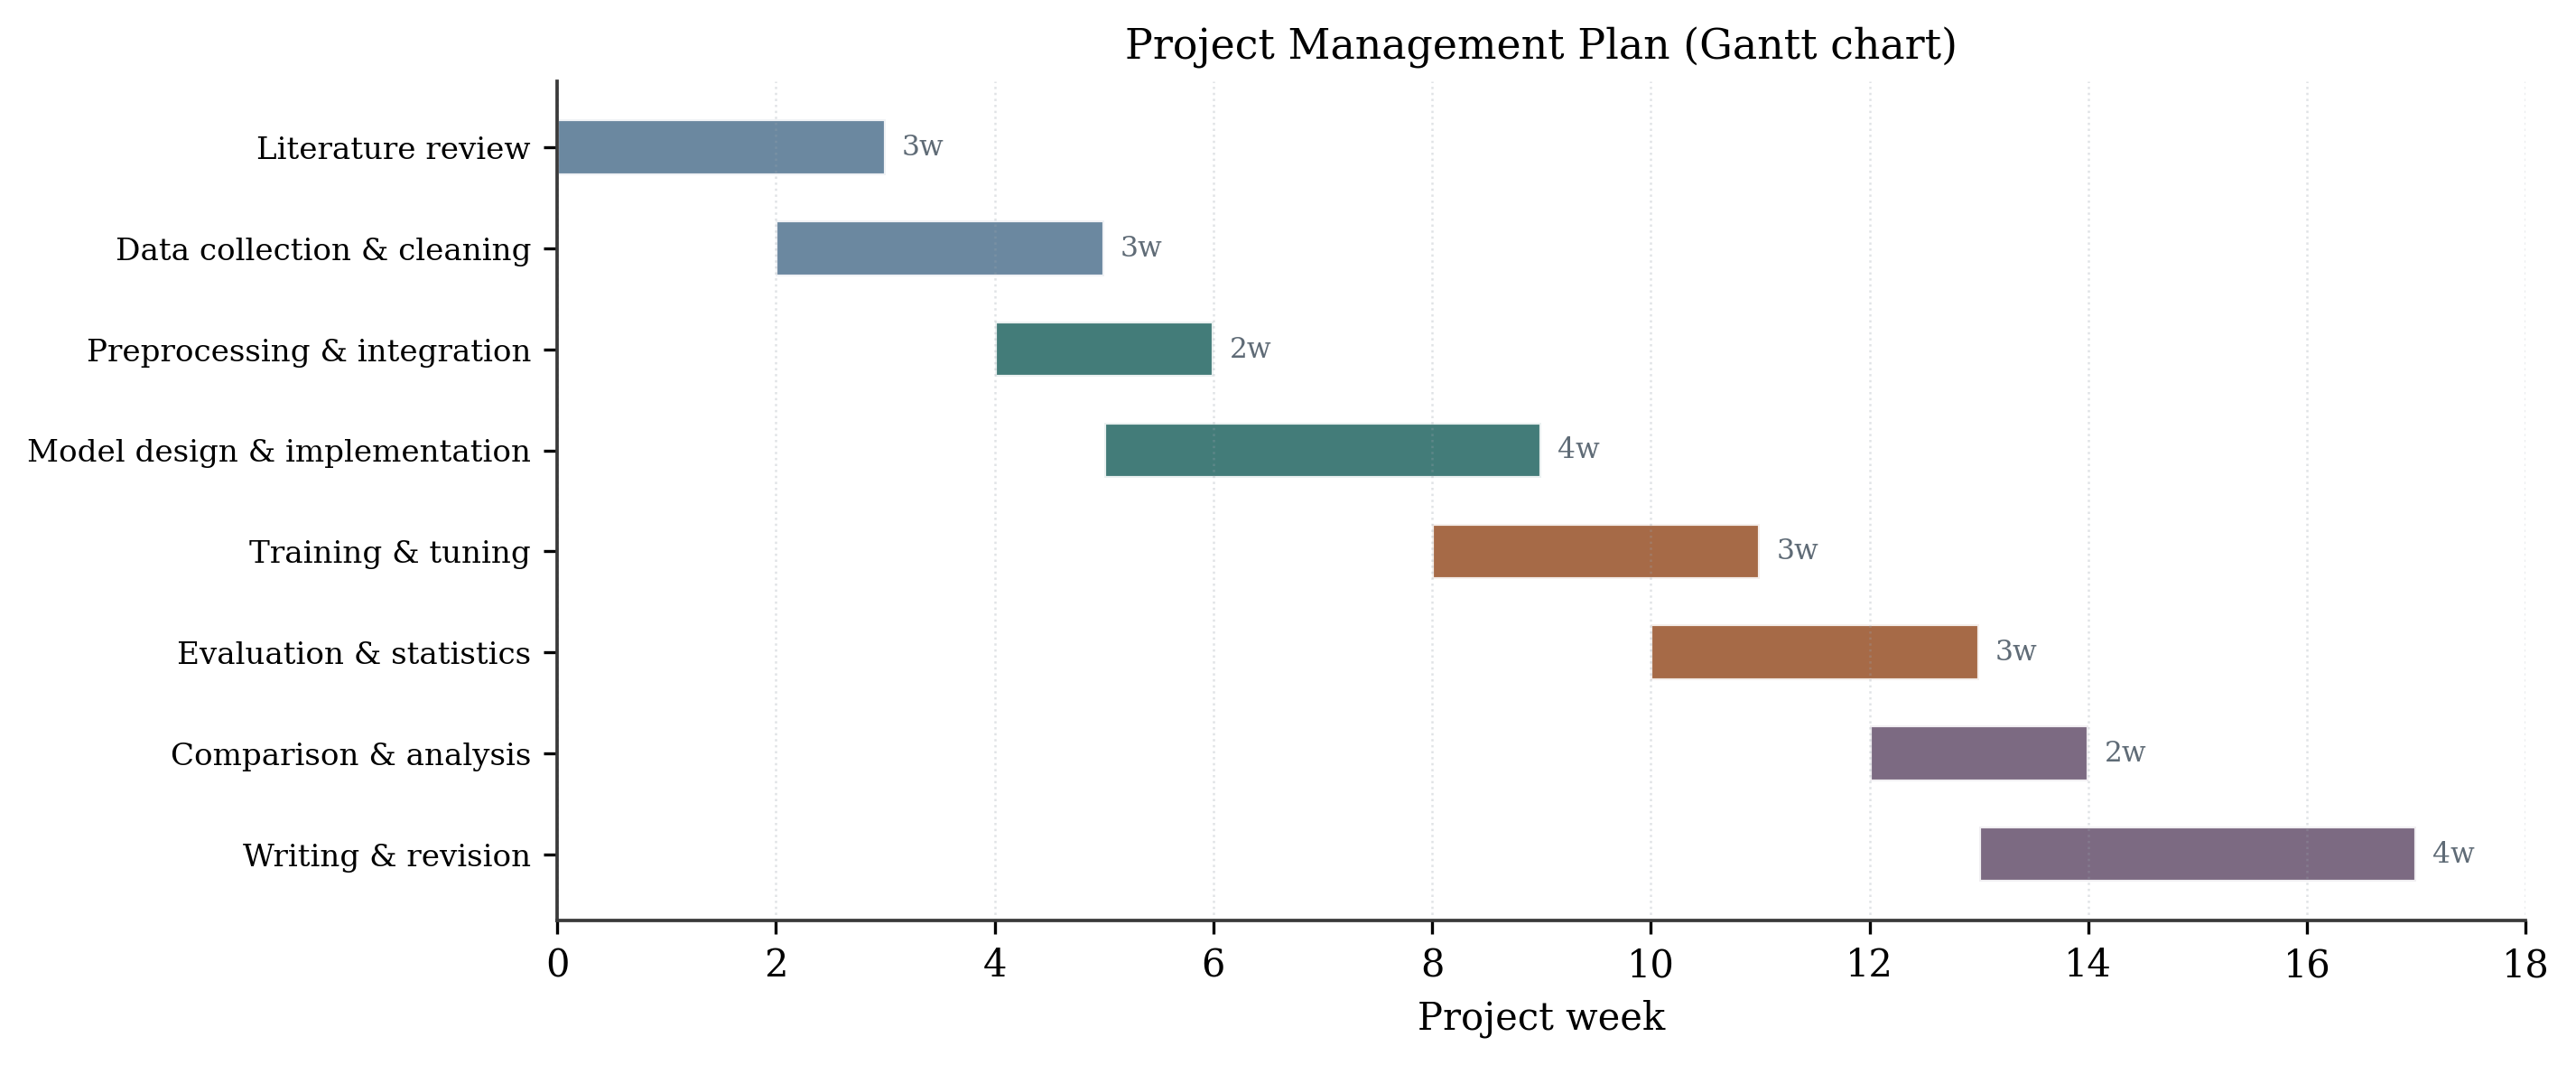
\includegraphics[width=\textwidth,keepaspectratio]{images/fig21_gantt.png}
\caption{Project management plan. Eight phases over an eighteen-week schedule, with deliberate overlap between data, modelling, and evaluation tasks.}
\label{fig:gantt}
\end{figure}

\section{Risk Management}
The six main risks were monitored on a likelihood–impact matrix (Fig.~\ref{fig:risk}). The highest-impact the calibrated ensemble and the calibrated ensemble combined with the direct response to risk (R4, overconfident hallucination) directly reduce risk.hallucination check, data related risks (R1 semi-synthetic trajectories, R2 class imbalance).compensated for by honest framing, and by reporting the calibration and coverage, rather than by relying on.The compact core coupled with a single LLM reduces the risk impacting cost and compute (R3, R5).Reproducibility (R6) is addressed by presenting all code and configurations, and call per query; and flexibility (R7) is addressed by releasing all code and configurations, which allows for easy and flexible use.

\begin{figure}[H]
\centering
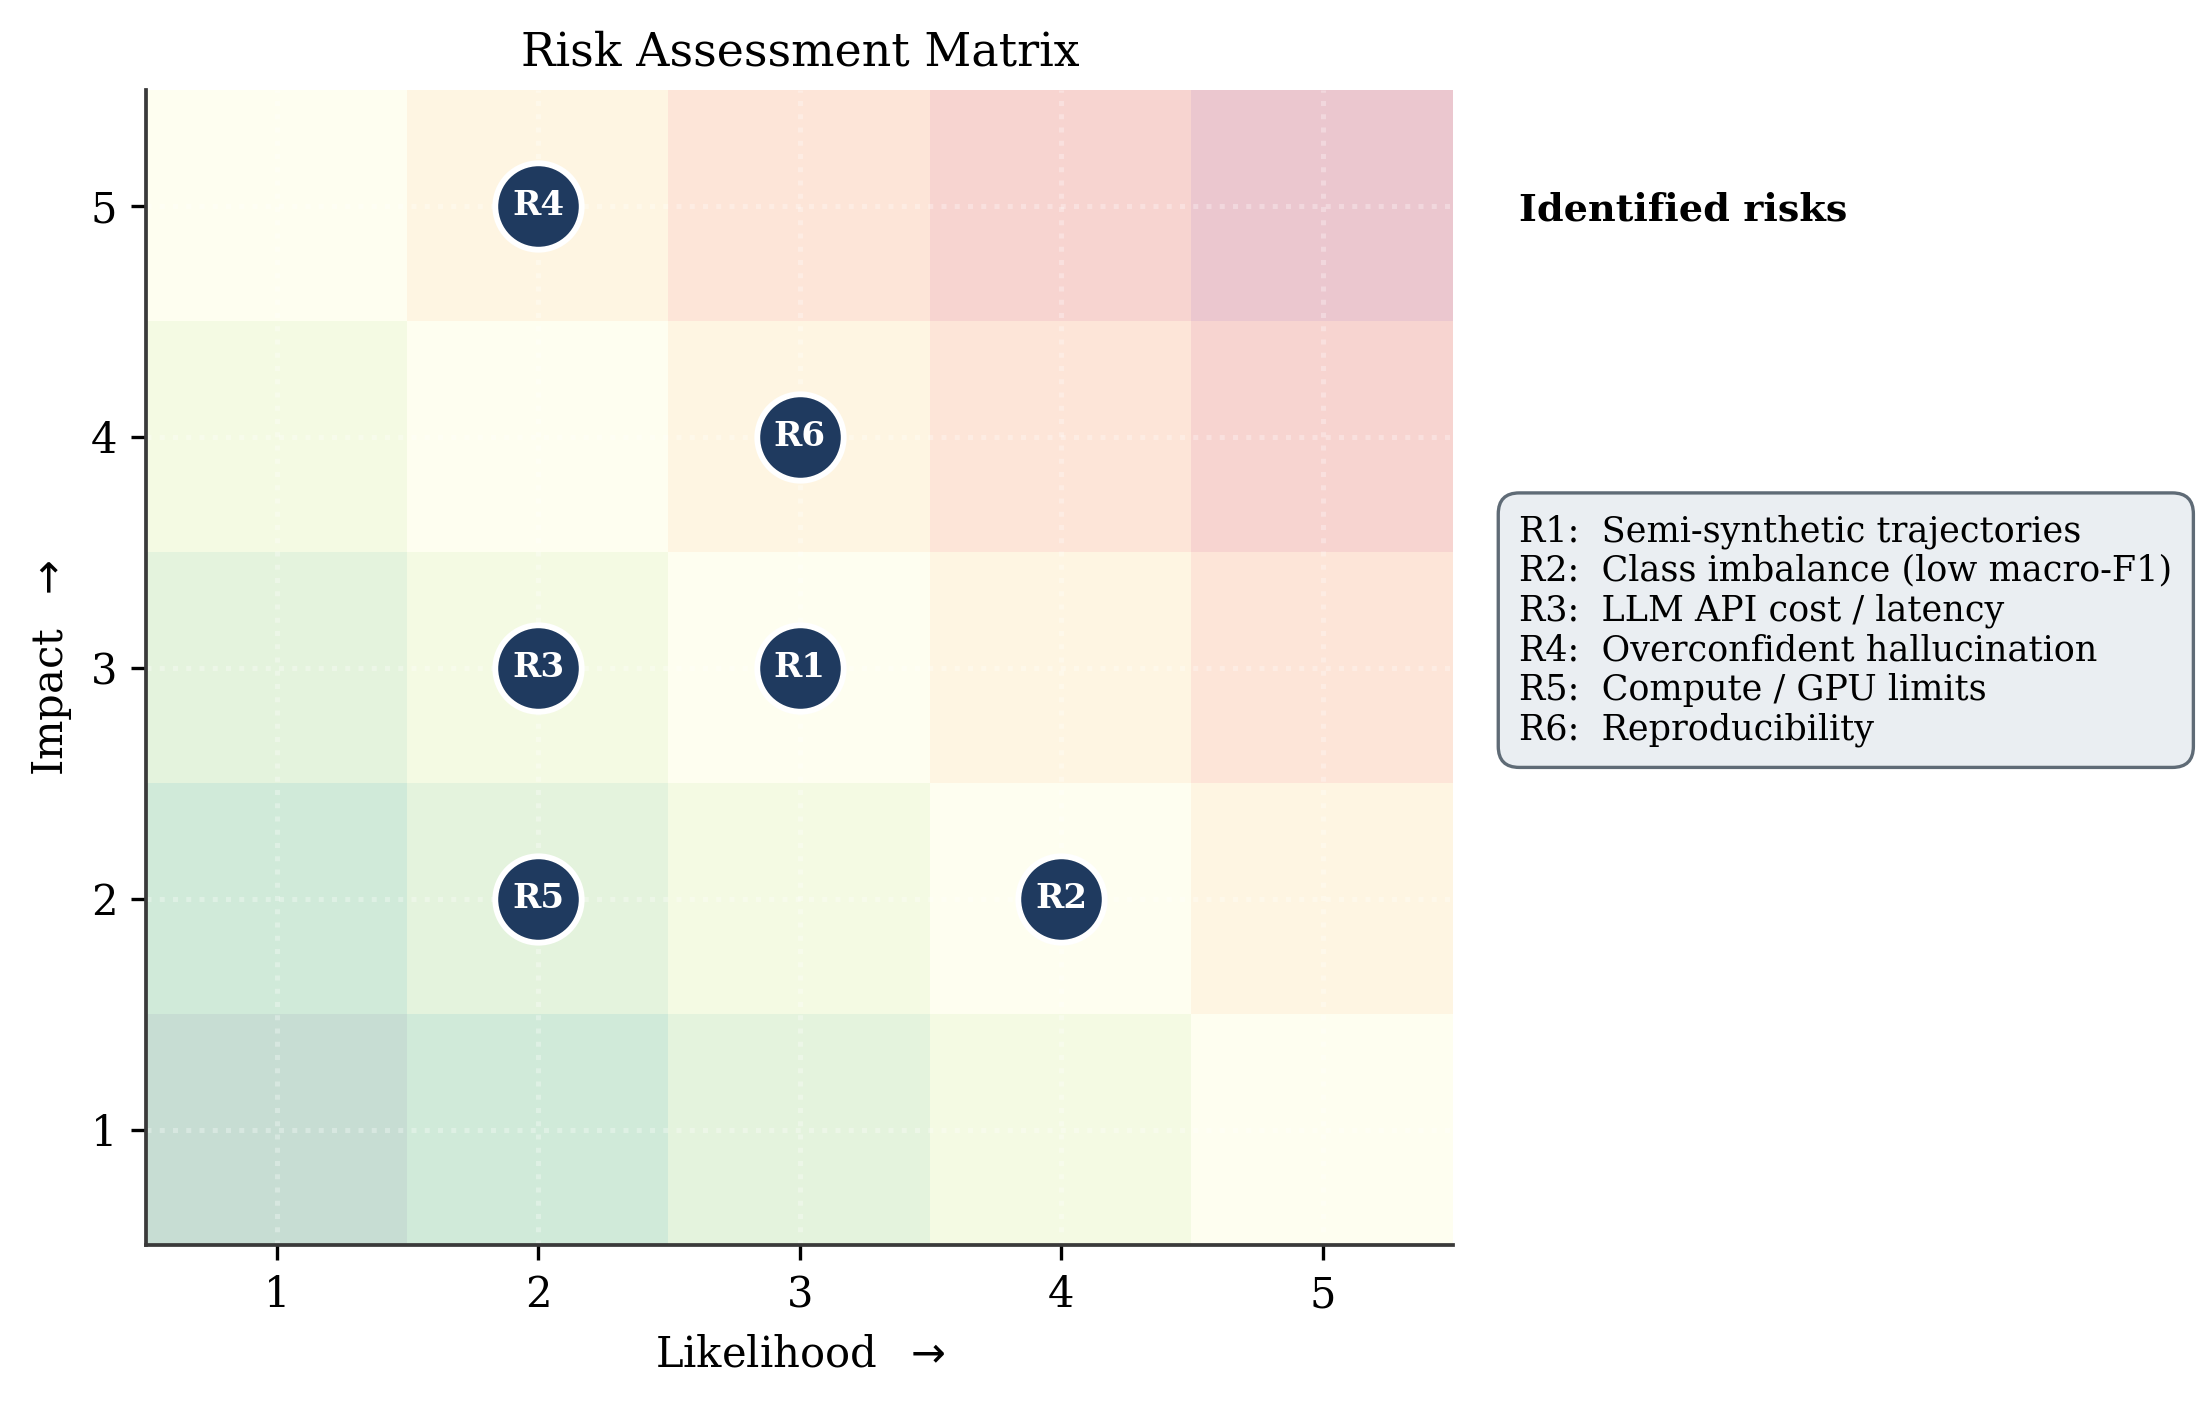
\includegraphics[width=0.85\textwidth,keepaspectratio]{images/fig22_risk_matrix.png}
\caption{Risk assessment matrix. Markers R1–R6 are positioned by likelihood and impact; the side legend names each risk. Mitigations are described in the text.}
\label{fig:risk}
\end{figure}



\section{Economic Analysis}
The external LLM api usage during evaluation is the majority of the direct project cost.The training period is short and the datasets are open (Fig.~\ref{fig:economic}a). The local core of the framework reduces the query cost compared to a design that only uses cloud-LLM due to the small local model absorbing the structured reasoning, while the remaining LLM call is for verbalisation (Fig.~\ref{fig:economic}b). The result is a favourable cost profile for a trustworthy answer.

\begin{figure}[H]
\centering
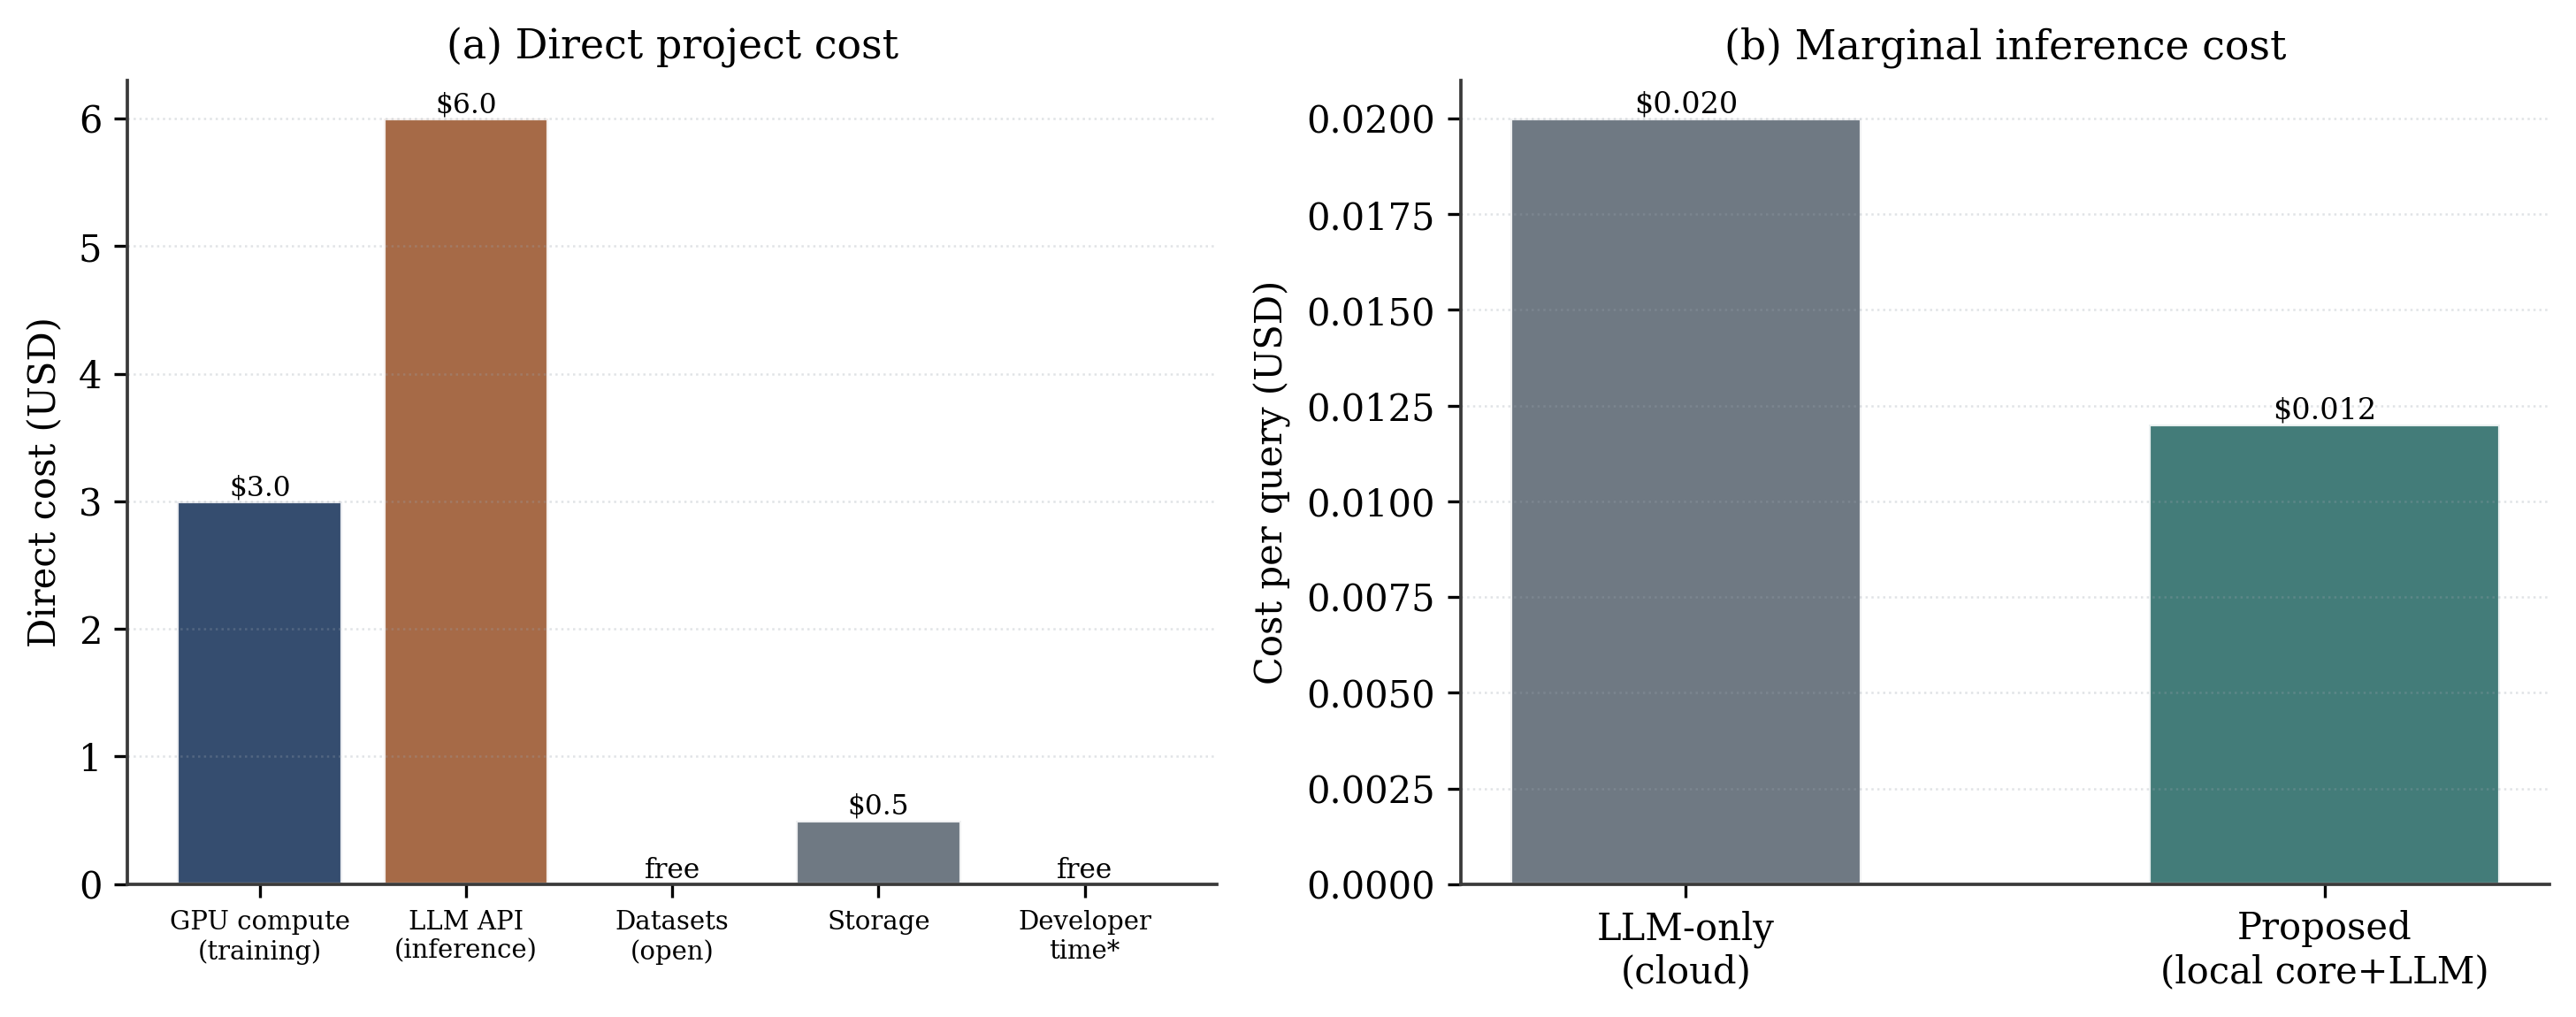
\includegraphics[width=\textwidth,keepaspectratio]{images/fig23_economic.png}
\caption{Economic analysis. (a) Direct project cost by category. (b) Marginal per-query inference cost of the proposed local-core-plus-LLM design versus a cloud-LLM-only baseline.}
\label{fig:economic}
\end{figure}